Localized excitations, or quanta, of the quantum fields in the SM are called elementary particles. Particles are observed either directly or indirectly through experiment and carry intrinsic properties that distinguish them from one another, such as electric charge, mass, and quantum numbers like spin. Every particle has a corresponding antiparticle, which, roughly speaking, is identical to the particle save for its carrying some opposite quantum numbers, e.g., electric charge for charged particles. All SM particles (and antiparticles) can be classified as either fermions or bosons, depending on their spin quantum number, detailed below in Sections~\ref{sec:Fermions} and~\ref{sec:Bosons}. Provided in Fig.~\ref{fig:SM} is a diagram of all the particles in the SM, practically organized, and includes a number of important properties for each; this diagram may be used as a map of the theory described in the following Sections.

\begin{figure}[H]
    \centering
    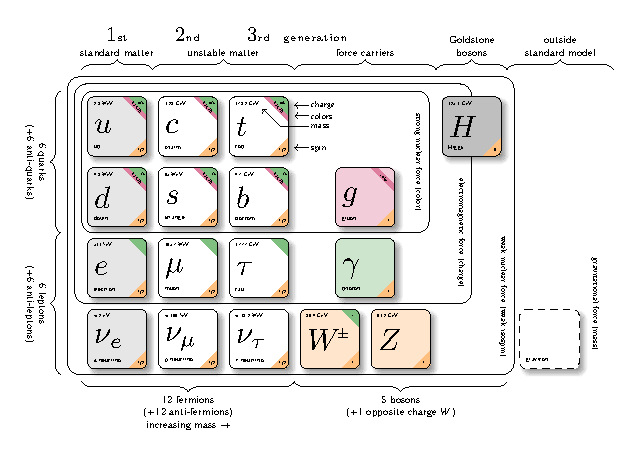
\includegraphics[width=1\textwidth]{Images/model-physics.pdf}
    \caption{Every elementary particle in the SM}
    \label{fig:SM}
\end{figure}

\subsubsection{Fermions} \label{sec:Fermions}
%fermions

Particles with half-integer spin quantum numbers obey Fermi-Dirac spin-statistics, which prevents any two identical particles from occupying the same state in a system at thermodynamic equilibrium, leading to the famous Pauli exclusion principle. Particles following a Fermi-Dirac distribution are given the eponymous name fermions, and while they are a general classification of any particle with half-integer spin, within the SM, fermions refer to a specific set of massive, interacting, ``matter'' particles that are subdivided into two key types: leptons and quarks. 

%leptons

Leptons $\ell$ are spin 1/2 fermions that can be electrically charged or neutral and interact via the weak nuclear force; they do not interact via the strong nuclear force (see Sections~\ref{sec:WeakInteraction} and~\ref{sec:StrongInteraction}). There are six types, or flavors, of leptons: the electron $e^-$, muon $\mu^-$, tau $\tau^-$, electron neutrino $\nu_e$, muon neutrino $\nu_{\mu}$, and tau neutrino $\nu_{\tau}$. These can be grouped into three generations: electronic, muonic, and tauonic, each with an electrically charged lepton and an electrically neutral lepton, dubbed a neutrino. Each lepton carrys a lepton family quantum number $L_e$, $L_{\mu}$, or $L_{\tau}$, equal to 1 ($-1$ for antileptons), that is approximately conserved (neutrino oscillations violate this). What is always conserved in interactions is lepton number $L = n_{\ell}-n_{\overline{\ell}}$, where $n_{\ell}$ and $n_{\overline{\ell}}$ are the number of leptons and antileptons at the start or end of an SM process.

An important characteristic of both fermions and bosons is their helicity, being the sign of the projection of a particle's spin onto its momentum: ``right-handed'' if the spin and momentum vectors align ($+1$), ``left-handed'' if the vectors are opposed ($-1$), denoted with an $R$ or $L$ subscript, respectively. In the limit where the particle is massless, helicity is essentially chirality, an intrinsic property of a particle that determines the representation it transforms under (for this reason we refer to left-handed and right-handed particles as chiral). Each generation of left-handed leptons form a weak isospin doublet with $T=1/2$:
\begin{equation}
    \left(\begin{array}{c}
        \nu_e \\
        e^-
    \end{array}\right)_L,
    \left(\begin{array}{c}
        \nu_{\mu} \\
        \mu^-
    \end{array}\right)_L,
    \left(\begin{array}{c}
        \nu_{\tau} \\
        \tau^-
    \end{array}\right)_L
\end{equation} 
while the right-handed leptons form singlets: $e^-_R$, $\mu^-_R$, $\tau^-_R$ with $T=0$. Note that there are no right-handed neutrinos in the SM, and that only left-handed leptons participate in charged weak interactions. For antileptons, the inverse is true: there are only right-handed antineutrinos and only right-handed charged antileptons participate in weak interactions.

Leptons are initially massless in the SM. Charged leptons aquire mass via the Higgs mechanism, while neutrinos remain massless. No neutrino mass has ever been measured (although upper bounds have been placed); however, observations of neutrino flavor oscillations confirm that neutrinos do indeed have very small masses, contrary to the SM. Table~\ref{tab:Leptons} lists for each lepton the flavor, spin, lepton family number, electric charge $Q$, weak isospin $T_3$, weak hypercharge $Y_W$, and observed mass (or upper bound on the mass for the neutrinos). There is a corresponding antiparticle for each lepton, where the charges are sign-flipped but retain the same mass.
\begin{table}[H]
    \begin{center}
        \caption{Quantum numbers and masses of the SM leptons. This table only lists the properties of left-handed leptons, with right-handed antileptons forming a similar table with the charges sign-flipped.}
        \begin{tabular}{lrrrrrrrl}
            \hline \hline
            Flavor          & Spin  & $L_e$ & $L_{\mu}$ & $L_{\tau}$    & $Q$   & $T_3$     & $Y_W$ & Obs. mass [MeV] \\ \hline
            $e$             & $1/2$ & $+1$   & $0$       & $0$           & $-1$   & $-1/2$    & $+1$  & \;\;\;\;$\num{0.511}$ \\
            $\mu$           & $1/2$ & $0$   & $+1$       & $0$           & $-1$   & $-1/2$    & $+1$  & \;\;\;\;$\num{105.7}$ \\
            $\tau$          & $1/2$ & $0$   & $0$       & $+1$           & $-1$   & $-1/2$    & $+1$  & \;\;\;\;$\num{1.777e3}$ \\
            $\nu_e$         & $1/2$ & $+1$   & $0$       & $0$           & $0$   & $+1/2$    & $-1$  & $<\num{2.2e-6}$ \\
            $\nu_{\mu}$     & $1/2$ & $0$   & $+1$       & $0$           & $0$   & $+1/2$    & $-1$  & $<\num{0.17}$ \\
            $\nu_{\tau}$    & $1/2$ & $0$   & $0$       & $+1$           & $0$   & $+1/2$    & $-1$  & $<\num{15.5}$ \\ \hline \hline
        \end{tabular}
        \label{tab:Leptons}
    \end{center}
\end{table}



%quarks

Quarks $q$ are chiral spin 1/2 fermions that carry fractional electric charge (in multiples of 1/3), weak isospin and weak hypercharge, and—--unique among the SM fermions---interact with the strong force. Analogous to lepton number, quarks carry a baryon quantum number $B$ of 1/3. Baryon number is strictly conserved in the SM, and---for any interaction---is defined as $3B=n_q-n_{\overline{q}}$, where $n_q$ and $n_{\overline{q}}$ are the number of quarks and antiquarks at the start or end of a process. Remarkably, quarks---identical to leptons---come in six flavors that can likewise be grouped into three generations (this unexplained parallel partly motivates the search for new physics in this thesis). The quark flavors are: up $u$ and down $d$ (first-generation), charm $c$ and strange $s$ (second-generation), and top $t$ and bottom $b$ (third-generation). Also, similar to leptons, quarks aquire mass via the Higgs mechanism. Table~\ref{tab:quarks} lists the quantum numbers and masses of each flavor of quark.
\begin{table}[H]
    \begin{center}
        \caption{Quantum numbers of quarks. Color charges are not considered. This table only lists the properties of quarks, with antiquarks forming a similar table with the charges sign-flipped.}
        \begin{tabular}{lrrrrrl}
            \hline \hline
            Flavor   & Spin  & $B$   & $Q$       & $T_3$     & $Y_W$   & Obs. Mass [MeV] \\ \hline
            up       & $1/2$ & $1/3$ & $+2/3$    & $-1/2$    & $+1/3$  & $\num{2.3}$ \\
            down     & $1/2$ & $1/3$ & $-1/3$    & $-1/2$    & $+1/3$  & $\num{4.8}$ \\
            charm    & $1/2$ & $1/3$ & $+2/3$    & $-1/2$    & $+1/3$  & $\num{1.274e3}$ \\
            strange  & $1/2$ & $1/3$ & $-1/3$    & $+1/2$    & $+1/3$  & $\num{9.5e1}$ \\
            top      & $1/2$ & $1/3$ & $+2/3$    & $+1/2$    & $+1/3$  & $\num{1.73210e5}$ \\
            bottom   & $1/2$ & $1/3$ & $-1/3$    & $+1/2$    & $+1/3$  & $\num{4.180e3}$ \\ \hline \hline
        \end{tabular}
        \label{tab:quarks}
    \end{center}
\end{table}

Each flavor of quark transforms as a color triplet under \SUthreeC, meaning it has a red, blue, or green color charge (antired, antiblue, or antigreen for antiquarks). As a quark absorbs or emits a gluon (carrying a color-anticolor charge), its color charge will change correspondingly. Quarks combine via the strong interaction to form color-neutral hadrons that are either a quark-antiquark pair called a meson (e.g., a pion) or a combination of three quarks called a baryon (e.g., the proton and the neutron). Color confinement restricts quarks inside of hadrons, and in the instance of a free quark (or gluon), QCD matter will spontaneously be pulled from the vacuum to neutralize the bare color charge, a process known as hadronization. Hard proton-proton collisions as seen in the LHC will often emit quarks, which must undergo hadronization repeatedly until all color fragments are neutralized, generating a slew of mesons and baryons all traveling within a tight cone with the momentum of the original quark. These cones of hadrons, colloquially called jets, are ubiquitous in collider experiments and are essential ingredients in many physics analyses. 


\subsubsection{Bosons} \label{sec:Bosons}
The spin statistics of particles with integer-valued spin quantum numbers follow a Bose-Einstein distribution, which allows an arbitrary number of identical particles to occupy quantum states and maintain thermal equilibrium (as opposed to Fermi-Dirac statistics). Particles with this behavior are naturally called a bosons. After the SM fermions, a collection of four SM bosons constitute the remainder of all observed fundamental particles. SM bosons can be massive or massless and are responsible for mediating the interactions between all particles. As the local gauge transformations of the SM are responsible for the fundamental interactions, the associated bosons are often called gauge bosons. In the SM there are three types of vector (spin 1) gauge bosons: the photon, the weak bosons, and the gluons; and one scalar (spin 0) boson: the Higgs boson. 

The photon is a massless spin 1 gauge boson that mediates the electromagnetic force, meaning it couples to any fermion with an electric charge (all but neutrinos). Photons themselves are uncharged, so they do not self-interact. The weak gauge bosons are also spin 1 and mediate the weak force. There are three kinds of weak gauge bosons: two charged, $W^+$ and $W^-$, and one neutral, $Z^0$. They are all massive, aquiring their masses via the Higgs mechanisim as explained in Section~\ref{sec:Higgs}. There are eight Gluons, massless spin 1 gauge bosons that mediate the strong force between particles with color charge, i.e., quarks. Gluons carry color charge and thus self-interact, leading to color confinemnt. The Higgs boson is a massive, complex scalar boson that is responsible for providing mass to the gauge bosons and SM fermions, through different mechanisms. The Higgs is theorized to self-interact and in 2012 was the last SM particle to be discovered. 
